\section{Sistema de telemetría}
\label{sec:telemetria}

El sistema de telemetría registra en tiempo real todos los eventos de una sesión de
producción: cambios de fuente activa, cambios de composite, activaciones del stream
blanker, estado de overlays y rótulos, niveles de audio y métricas de rendimiento del
servidor. Esta información permite tanto la monitorización durante el directo como la
auditoría posterior de la sesión.

\subsection{Arquitectura del servicio}

El servicio (\texttt{telemetry\_service.py}) es un proceso Python independiente que
se conecta al puerto 9999 de voctocore como un cliente TCP ordinario, sin requerir
privilegios especiales. Al conectarse, envía el comando \texttt{get\_config} para
obtener los parámetros del pipeline: resolución, framerate, formato de píxel y
configuración de audio. Estos datos se incluyen en el campo \texttt{stream\_info} de
cada entrada del log, dotando al registro de validez técnica para análisis de rendimiento.

A continuación, el servicio escucha continuamente los mensajes del protocolo interno
de voctocore, filtrando los eventos relevantes: \texttt{video\_status} (fuentes activas
en programa y preview), \texttt{composite\_mode} (distribución de pantalla activa) y
\texttt{stream\_status} (LIVE, PAUSE, NOSTREAM).

Voctocore desconoce el estado de los elementos gestionados exclusivamente en la
interfaz gráfica, como los rótulos dinámicos o los niveles de los faders de audio.
Para capturar esta información sin modificar el núcleo, el módulo
\texttt{gui\_state\_exporter.py} de voctogui recorre el árbol de widgets GTK de forma
segura para hilos y exporta periódicamente el estado completo de la interfaz. En modo
local, escribe el fichero \texttt{sessions/gui\_state.json}; en modo red (Docker o dos
PCs), lo envía mediante HTTP POST al servicio de telemetría. El servicio fusiona ambas
fuentes de datos, protegidas por cerrojos de hilo, para construir una vista unificada
del sistema.

Para identificar el origen de los comandos en escenarios distribuidos, el servicio
determina la IP de red de forma automática: en entornos Docker lee la variable de
entorno \texttt{HOST\_IP} inyectada por Docker Compose; en modo nativo, abre un socket
UDP hacia \texttt{8.8.8.8} sin llegar a establecer conexión efectiva, lo que permite
consultar la tabla de enrutamiento del kernel y obtener la IP real de la interfaz de
salida.

\subsection{Registro y métricas}

El registro sigue una doble vía temporal:

\begin{itemize}
  \item \textbf{Por evento (\texttt{CHANGE}):} cuando se detecta cualquier variación
        de estado, la entrada se escribe inmediatamente con su marca de tiempo,
        capturando cada corte o cambio de composite en el instante exacto en que ocurre.
  \item \textbf{Por latido (\texttt{STATE}):} un hilo paralelo escribe el estado
        completo del sistema cada 5~segundos como medida de redundancia, independientemente
        de que haya habido cambios.
\end{itemize}

Cada entrada incluye un bloque \texttt{system\_health} con las siguientes métricas del
servidor:

\begin{itemize}
  \item \textbf{CPU (\texttt{cpu\_usage\_percent}):} calculado a partir de
        \texttt{/proc/stat}. Si supera el 80\,\%, GStreamer comienza a descartar
        fotogramas, degradando la emisión.
  \item \textbf{Memoria (\texttt{ram\_usage\_percent}, \texttt{ram\_available\_mb}):}
        leído de \texttt{/proc/meminfo}. Un valor bajo y estable confirma que los
        pipelines GStreamer procesan y liberan fotogramas en tiempo real sin acumular
        búferes.
  \item \textbf{Ancho de banda por cámara:} calculado como
        $\text{Mbps} = \frac{W \times H \times \text{FPS} \times 12}{1\,000\,000}$,
        donde 12 bits es la profundidad de color del formato I420 (YUV420p). Para
        1080p25 el resultado es aproximadamente 622~Mbps por fuente, lo que confirma
        que todo el tráfico de vídeo debe circular en bucle local sin atravesar
        interfaces físicas convencionales.
  \item \textbf{Tiempos (\texttt{uptime}, \texttt{session\_duration}):} permiten
        correlacionar los cortes del log con el código de tiempo del archivo de
        grabación final.
\end{itemize}

Las entradas se escriben en formato \textit{JSON Lines} (\texttt{session\_N.jsonl}):
un objeto JSON completo por línea, con numeración automática por sesión. Este formato
permite leer el log de forma incremental con herramientas estándar (\texttt{jq},
Python) sin necesidad de cargar el fichero completo en memoria.

Un ejemplo de entrada de tipo CHANGE tras un corte de cámara:

\begin{verbatim}
{"timestamp": "2025-03-28 20:14:32",
 "type": "change",
 "output":  {"channel_a": "cam2", "channel_b": "cam1"},
 "preview": {"channel_a": "cam1", "channel_b": "cam2"},
 "mode": "live",
 "composite": {"name": "full_screen", "fullscreen": true},
 "audio": {"cam1_db": -12.0, "cam2_db": 0.0},
 "system_health": {"cpu_usage_percent": 34.2, "ram_usage_percent": 8.7,
                   "calc_bandwidth_mbps_per_cam": 622.08},
 "stream_info": {"video_resolution": "1920x1080", "video_fps": "25",
                 "video_pix_fmt": "I420"}}
\end{verbatim}

\subsection{API REST y mensajería AMQP}

El servicio expone los datos de telemetría en dos canales complementarios:

\begin{itemize}
  \item \textbf{API REST HTTP (puerto 8080):} implementada con la librería estándar de
        Python sin dependencias externas. Devuelve el estado actual completo en formato
        JSON. La opción \texttt{allow\_reuse\_address} evita bloqueos de puerto en
        reinicios rápidos del servicio.
  \item \textbf{Mensajería AMQP~\cite{oasis_amqp10} (RabbitMQ~\cite{rabbitmq_docs}):} cada cambio de estado se publica en el
        exchange \texttt{voctomix\_events} (tipo fanout), de forma que cualquier
        consumidor externo puede suscribirse a los eventos sin acoplarse directamente
        al servicio de telemetría ni a voctocore.
\end{itemize}

\subsection{RabbitMQ como broker de mensajería}
\label{sec:rabbitmq}

RabbitMQ es el broker AMQP que centraliza los eventos de telemetría. En el despliegue
Docker se ejecuta como un contenedor independiente en los puertos 5672 (AMQP) y 15672
(consola web de administración).

La integración con RabbitMQ permite mantener un registro persistente de todos los
eventos con marca de tiempo para análisis posterior, conectar Voctomix con sistemas
externos de monitorización o automatización (ELK Stack, Grafana), y verificar durante
las pruebas que cada acción del realizador genera el evento correspondiente.

En el marco del proyecto europeo de investigación CyberNEMO (UPM), el broker RabbitMQ
de Voctomix~2.0 fue integrado en el clúster Kubernetes del proyecto, donde las colas
\texttt{vproduction-uc-media} y \texttt{vqprobe-uc-media} recibieron los eventos del
mezclador en tiempo real durante las pruebas de producción audiovisual. Este despliegue
constituyó la primera validación del sistema de telemetría en un entorno real.

\begin{figure}[H]
  \centering
  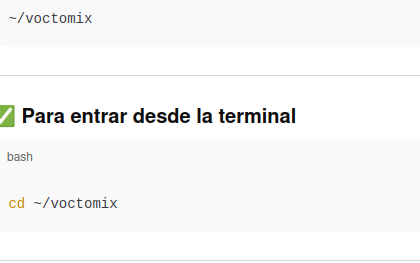
\includegraphics[width=\textwidth]{figuras/rabbitmq_cybernemo_queues.png}
  \caption{Colas RabbitMQ activas durante la integración con CyberNEMO.}
  \label{fig:rabbitmq_cybernemo}
\end{figure}

La arquitectura desacoplada del servicio, conectado al núcleo como un cliente TCP
ordinario sin privilegios especiales, garantiza que su eventual fallo no afecte al
procesamiento multimedia principal.

\subsection{Evolución del protocolo: de UDP a HTTP}
\label{sec:evolucion_telemetria}

En el escenario de dos PCs, el servicio de telemetría necesita recibir el estado de la
GUI desde el PC del realizador a través de la red. La implementación inicial utilizó
UDP, que presentó dos problemas críticos:

\begin{itemize}
  \item \textbf{Falta de fiabilidad:} UDP es \textit{fire-and-forget}; los paquetes
        de estado podían perderse sin que el emisor lo detectara, dejando el servicio
        y la GUI desincronizados.
  \item \textbf{Bloqueos de puerto (\texttt{Errno 98}):} al reiniciar los scripts
        rápidamente durante el desarrollo, el kernel mantenía el puerto en estado
        \texttt{TIME\_WAIT}, impidiendo el rearranque inmediato del servicio.
\end{itemize}

La solución fue migrar a HTTP/TCP: el servicio actúa como servidor HTTP en el puerto
8080, y \texttt{gui\_state\_exporter.py} envía los datos mediante peticiones HTTP POST
con cuerpo JSON. TCP garantiza la entrega ordenada de los datos, y se estableció un
\textit{timeout} de 1~segundo en el cliente para que la GUI nunca se bloquee si el
servidor no está disponible.
